\documentclass[11pt]{beamer}
\usepackage{fontspec}
\setmainfont{Times New Roman}

\usepackage[spanish,es-tabla]{babel}
\usepackage{multimedia}
%\usepackage{epstopdf}
\usepackage{longtable,multirow,booktabs}
\usepackage[dvipsnames,table]{xcolor}
\usepackage{tabularx}
\usepackage{adjustbox}
\usepackage{tcolorbox}
\usepackage{amsmath,amsfonts,amssymb,graphicx}
\usepackage{ragged2e}
\usepackage{hyperref}
\usepackage{tikz}
\usetikzlibrary{arrows.meta, positioning, shapes.geometric, shapes, calc}
\usepackage{wrapfig}
\usepackage{subcaption}
\usepackage{graphicx}
\usepackage{caption}
\usepackage{xlop}
\usepackage{multicol}

\useoutertheme{smoothbars}
\useinnertheme{rounded}

\definecolor{color1}{RGB}{192,72,72}
\definecolor{color2}{RGB}{0,0,120}
\definecolor{color3}{RGB}{0,0,255}
\definecolor{color4}{RGB}{5,5,5}
\definecolor{color5}{RGB}{255,160,160}

\definecolor{mygreen1}{RGB}{0,73,44}
\definecolor{mygreen2}{RGB}{0,140,81}
\definecolor{mygreen3}{RGB}{0,208,120}

\definecolor{verde_kaki}{RGB}{100,100,0}

\setbeamertemplate{navigation symbols}{}

\definecolor{light-gray}{HTML}{E5E4E2}
\definecolor{light-cyan}{HTML}{E0FFFF}

\newtcolorbox{mybox}[1]
{colback=coral!5!white,colframe=coral!75!black,fonttitle=\bfseries,title=#1}

\setbeamercolor{structure}{fg=white,bg=mygreen2}
\setbeamercolor*{palette primary}{fg=mygreen1,bg=mygreen2}
\setbeamercolor*{palette secondary}{fg=white,bg=mygreen1}
\setbeamercolor*{palette tertiary}{bg=mygreen1,fg=white}
\setbeamercolor*{palette quaternary}{fg=white,bg=mygreen2!50}

\setbeamercolor{frametitle}{fg=white!90!mygreen1}

\setbeamercolor{section in head/foot}{fg=white,bg=mygreen1}
\setbeamercolor{group in head/foot}{fg=white,bg=mygreen3}
\setbeamercolor{title in head/foot}{fg=white,bg=mygreen2}

\defbeamertemplate*{headline}{mytheme}
{%
  \begin{beamercolorbox}[ht=2.25ex,dp=3.75ex]{section in head/foot}
    \insertnavigation{\paperwidth}
  \end{beamercolorbox}%
}%
\subtitle[ICAR, ETSIIT, UGR]{Trabajo final}
\newcommand{\myMateria}{Servidores Web de Altas Prestaciones}
\defbeamertemplate*{footline}{mytheme}
{
  \leavevmode%
  \hbox{%
  \begin{beamercolorbox}[wd=.4\paperwidth,ht=3ex,dp=1ex,center]{section in head/foot}%
    \usebeamerfont{section in head/foot}\myMateria
  \end{beamercolorbox}%
  \begin{beamercolorbox}[wd=.25\paperwidth,ht=3ex,dp=1ex,center]{title in head/foot}%
    \usebeamerfont{title in head/foot} \insertsubtitle
  \end{beamercolorbox}%
    \begin{beamercolorbox}[wd=.35\paperwidth,ht=3ex,dp=1ex,center]{group in head/foot}%
    \usebeamerfont{group in head/foot}\hspace{0.6cm}\insertshortsubtitle \hspace{0.8cm}
    \insertframenumber{} / \inserttotalframenumber
  \end{beamercolorbox}}%
  \vskip0pt%
}

\title{ \textit{Granja de modelos de IA}}
\author{Francisco Javier Pérez García \\ \and Manuel Ruiz Aguilar \\ \and Gabriel Francisco Sánchez Muñoz }
\date{\textit{\textcolor{mygreen2}{\myMateria, \insertshortsubtitle}}}

 
\begin{document}

\begin{frame}
\maketitle
\end{frame}

\section{Introducción}
\begin{frame}
\frametitle{Introducción}
\begin{figure}[H]
    \centering
    \begin{subfigure}[H]{0.27\textwidth}
        \centering
        
\includegraphics[width=\textwidth]{Images/ollama.png}
    \end{subfigure}
    \hfill
    \begin{subfigure}[H]{0.42\textwidth}
        \centering
        
\includegraphics[width=\textwidth]{Images/docker.png}
    \end{subfigure}
\end{figure}
\begin{center}
{\Huge
\textbf{¿IA + Granja?}
}
\end{center}

\end{frame}

\section{Fundamentos}
\begin{frame}
\frametitle{Fundamentos}
\begin{itemize}
    \item \textbf{Docker y Docker Compose}: Contenerización.
    \item \textbf{Ollama + Qwen3.5 0.8b}: Software para ejecutar modelos IA.
    \item \textbf{LiteLLM}: Balanceador para IAs.
    \item \textbf{Redis Stack}: Almacenamiento de caché semántico.

\[ \text{sim}(\vec{a}, \vec{b}) = \frac{\vec{a} \cdot \vec{b}}{\|\vec{a}\| \cdot \|\vec{b}\|} \in [-1, 1] \]

    \item \textbf{Nginx}: Proxy inverso.
    \item \textbf{Locust y Python}: Test de funcionalidad.
\end{itemize}

\end{frame}

\section{Objetivos}
\begin{frame}
\frametitle{Objetivos}
\begin{enumerate}
    \item Granja IA organizada por funcionalidad y reproducible.
    
    \item Distribuir trabajo con balanceo de carga.
    
    \item Reducir la carga con consulta al caché semántico.
    
    \item Usar un proxy de alto rendimiento con respuestas en \emph{streaming}.
    
    \item Realizar mediciones del rendimiento.
\end{enumerate}
\end{frame}

\section{Arquitectura}
\begin{frame}{Arquitectura}
    
    \begin{figure}[H]
        \centering
        \shorthandoff{>}\shorthandoff{<}
        \scalebox{0.48}{%
        \begin{tikzpicture}[
            node distance=1.8cm and 1.2cm,
            box/.style={rectangle, draw=black!60, fill=black!5, very thick, minimum width=2.8cm, minimum height=1cm, align=center},
            db/.style={cylinder, draw=black!60, fill=black!5, very thick, minimum width=2cm, minimum height=1cm, align=center, shape border rotate=90},
            arrow/.style={-stealth, thick}
        ]
            \node[font=\sffamily\bfseries, box, fill=color5!30] (cliente) {Cliente\\externo};
            
            \node[font=\sffamily\bfseries, box, right=of cliente] (nginx) {Nginx\\:80};
            
            \node[font=\sffamily\bfseries, box, right=of nginx] (litellm) {LiteLLM\\:4000};
            
            \node[font=\sffamily\bfseries, db, above=of litellm, yshift=-0.5cm] (redis) {Redis Stack\\:6379};
            
            \node[font=\sffamily\bfseries, box, below left=of litellm, yshift=0.5cm, xshift=-1cm] (ollama1) {Ollama-1\\:11434\\(qwen3.5)};
            \node[font=\sffamily\bfseries, box, below right=of litellm, yshift=0.5cm, xshift=1cm] (ollama2) {Ollama-2\\:11436\\(qwen3.5)};
            
            \node[font=\sffamily\bfseries, box, above=of redis, yshift=-0.5cm] (ollamaEmb) {Ollama-embed\\:11435\\(nomic-embed)};
            
            \draw[arrow] (cliente) -- (nginx);
            \draw[arrow] (nginx) -- (litellm);
            \draw[arrow] (litellm) -- (redis) node[font=\sffamily\bfseries, midway, right] {cache};
            \draw[arrow] (litellm) -- (ollama1) node[font=\sffamily\bfseries, midway, left] {infer};
            \draw[arrow] (litellm) -- (ollama2) node[font=\sffamily\bfseries, midway, right] {infer};
            \draw[arrow] (litellm) -- (ollamaEmb) node[font=\sffamily\bfseries, midway, right, yshift=2.6cm] {embed};
            \draw[arrow, densely dashed] (redis) -- (ollamaEmb);
        \end{tikzpicture}%
        }
        \caption{Arquitectura del sistema: flujo de peticiones entre componentes.}
        \label{fig:arquitectura}
    \end{figure}
    
\end{frame}

\section{Implementación}
\begin{frame}
\frametitle{Implementación}
\begin{itemize}
    \item \textbf{\texttt{docker-compose.yml}}: red \emph{semantic-cache-net}, \emph{depends\_on}, puertos, comandos, variables de entorno, scripts, healthchecks y volúmenes.

    \item \textbf{\texttt{configv2.yaml}}: dos entradas para inferencia y una para embeddings, con sus debidos parámetros de APIs, el umbral de similitud a 0.85, tamaño de vector y tiempo de vida en caché.

    \item \textbf{\texttt{nginx.conf}}: redirige a LiteLLM:4000, permite \emph{streaming} y extiende timeouts.
\end{itemize}

\end{frame}

\section{Análisis de rendimiento}
\subsection{Resultados}
\begin{frame}{Análisis de rendimiento}{Resultados de \texttt{test\_litellm.py}}
\begin{table}[H]
    \centering
    \caption{HITs esperados (w) y obtenidos (r).}
    \label{tab:resultados}
    \hspace{-0.2cm}

    \begin{tabular}{lcccc}
        \toprule
        \textbf{Grupo} & \textbf{Pet.} & \textbf{HITs (w)} & \textbf{HITs (r)} & \textbf{Acierto} \\
        \midrule
        Duplicados exactos      & 20 & 10 & 10 & 100\,\% \\
        Paráfrasis Geografía    & 15 & 10 & 10 & 100\,\% \\
        Paráfrasis Ciencia      & 15 & 10 &  4 &  40\,\% \\
        Paráfrasis Historia     & 15 & 10 &  7 &  70\,\% \\
        Relacionados distintos  &  9 &  0 &  0 &   --- \\
        No relacionados         &  5 &  0 &  1 & ---    \\
        Balanceo de carga       & 10 &  0 &  0 & ---    \\
        \bottomrule
    \end{tabular}

\end{table}

\end{frame}
\begin{frame}{Análisis de rendimiento}{Resultados de \texttt{test\_litellm.py}}

\begin{figure}[H]
    \centering
    % Primera subfigura

    %\hspace{-1cm}
    \begin{subfigure}[H]{0.48\textwidth}
        \centering
        \shorthandoff{>}\shorthandoff{<}
        \scalebox{0.64}{%
        \begin{tikzpicture}
            \draw[fill=green!40]  (0,0)    rectangle (2.5,0.2)  node[midway] {31 ms};
            \draw[fill=red!40]    (3.5,0)  rectangle (6.0,5.9)  node[midway] {5929 ms};
            \node[anchor=west] at (0,-0.6)   {Cache HIT};
            \node[anchor=west] at (3.5,-0.6) {Cache MISS};
            \node[anchor=north] at (3,-1.4)  {Factor de aceleraci\'on: $191.5\times$};
            \draw[-stealth] (-0.5,0) -- (7,0);
            \node[anchor=north east] at (7,0.2) {ms};
        \end{tikzpicture}%
        }
        \label{fig:latencia}
    \end{subfigure}
    \hfill
    \begin{subfigure}[H]{0.50\textwidth}
        \centering
        \shorthandoff{>}\shorthandoff{<}
        \scalebox{0.66}{%
        \begin{tikzpicture}
            \draw[fill=blue!40]   (0,0)   rectangle (2.5,4.5) node[midway] {45 req};
            \draw[fill=orange!40] (3.5,0) rectangle (6.0,4.4) node[midway] {44 req};
            \node[anchor=west] at (0,-0.6)   {ollama-1 (51\,\%)};
            \node[anchor=west] at (3.5,-0.6) {ollama-2 (49\,\%)};
            \draw[-stealth] (-0.5,0) -- (7,0);
            \node[anchor=north east] at (7,0.2) {peticiones};
        \end{tikzpicture}%
        }
        \label{fig:balanceo}
    \end{subfigure}
\end{figure}%

\end{frame}

\subsection{Resultados}
\begin{frame}{Análisis de rendimiento}{Resultados de \texttt{locustfile.py}}
\begin{table}[H]
    \centering
    \label{tab:resultados2}
    \hspace{-0.2cm}
\small
  \begin{tabularx}{\textwidth}{lrrrrrr}
  \toprule
  \textbf{Grupo} & \textbf{Pets.} & \textbf{50\%} & \textbf{Media}& \textbf{Mín.} & \textbf{Máx.} & \textbf{Av. Tam.} \\
  \midrule
  Duplic. exactos & 129 & 310 & 3780 & 45 & 52933 & 308 \\
  Balanceo de carga  & 12 & 28000 & 25615 & 12583 & 44469 & 281 \\
  Paráfrasis Geo& 24 & 250 & 9864 & 56 & 52635 & 304 \\
  Paráfrasis Hist & 28 & 880 & 8357 & 59 & 37526 & 300 \\
  Paráfrasis Ciencia & 40 & 250 & 7619 & 57 & 47966 & 303 \\
  Relac. distintos & 23 & 1400 & 13803 & 60 & 44017 & 298 \\
  No relacionados & 15 & 410 & 8302 & 60 & 59903 & 305 \\
  \bottomrule
  \end{tabularx}

\end{table}

\end{frame}

\begin{frame}{Análisis de rendimiento}{Resultados de \texttt{locustfile.py}}
\begin{figure}[H]
  \begin{center}
    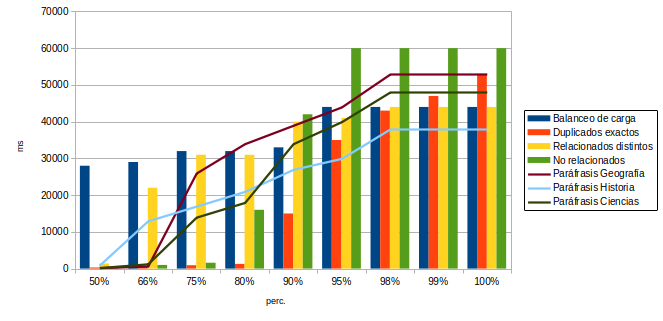
\includegraphics[width=\textwidth]{Images/graf_perc.png}
  \end{center}
\end{figure}
\end{frame}

\section{Conclusiones}
\begin{frame}{Conclusiones}{Cumplimiento de objetivos}
\begin{table}[H]
    \centering

    \begin{tabular}{p{5cm}|p{5.5cm}}
        \toprule
        \textbf{Cumplido} & \textbf{Limitación}  \\
        \midrule
        Aceleración de 191.5x en latencia con caché. & El umbral fijo no se adapta completamente.\\ \hline
        Buena detección de paráfrasis en dominios con vocabulario diferenciado.  & En ciencia; por ejemplo; no.    \\ \hline
        Balanceo equitativo.  & Contamos solo con 2 réplicas de inferencia.   \\ \hline
        Cambios en la configuración independientes y sencillos. & La latencia se limita con la CPU y se aumenta con el paso intermedio de consultar caché. \\ \hline
        Puede atender al menos dos peticiones por segundo. & ---  \\ 
        \bottomrule
    \end{tabular}

\end{table}
\end{frame}

\begin{frame}{Conclusiones}{Trabajo futuro}
\begin{itemize}
    \item Umbral adaptativo.
    \item Caché multinivel.
    \item Más réplicas, con escalado dinámico.
    \item Aceleración por hardware.
    \item Monitorización con Prometheus y Grafana.
    \item Nuevo test de carga.
\end{itemize}

\vspace{0.2cm}
Red:

\begin{itemize}
    \item Reglas según IP.
    \item Certificado SSL en Nginx.
    \item Optimización de envío según parámetros concretos.
\end{itemize}

\end{frame}

\begin{frame}
    \begin{center}
    {\Huge
    \textbf{FIN}
    }
    \end{center}
\end{frame}

\end{document}